\documentclass{beamer}
\usetheme{Madrid}
\colorlet{beamer@blendedblue}{green!40!black}
\setbeamertemplate{caption}[numbered]
\usepackage{amssymb, amsmath, amsthm}
\usepackage{physics}
\usepackage{float, subcaption, graphicx}
\usepackage{hyperref}

\title{Chapter 1 - Fusion}
\author{Hunt Feng\inst{1}}
\institute[Usask]
{
	\inst{1}%
	Faculty of Physics And Engineering Physics\\
	University of Saskatchewan
}
\date{\today}

%%%%%%%%%%%%%%%%%%%%
% section page 
%%%%%%%%%%%%%%%%%%%%
\AtBeginSection[]
{
	\begin{frame}{Outline of Presentation}
		\tableofcontents[currentsection]
	\end{frame}
}

\begin{document}
%%%%%%%%%%%%%%%%%%%%
% title and TOC
%%%%%%%%%%%%%%%%%%%%
\maketitle
\begin{frame}{Outline of Presentation}
	\tableofcontents
\end{frame}

%%%%%%%%%%%%%%%%%%%%
% contents 
%%%%%%%%%%%%%%%%%%%%
\section{Introduction to Fusion}
\begin{frame}{Fusion Reactions}
	There are a few fusion reactions,
	\begin{itemize}
		\item D-T reaction: large cross-section at low temperature, but hard to find Tritium.
		      \[ ^2_1D + ^2_1T \rightarrow ^4_2He + ^1_0n + 17.6\text{MeV} \]
		\item D-D reaction: easy to find the fuel, but small cross-section at low temperature.
		      \[ ^2D + ^2D \rightarrow ^3He + ^1n + 3.27\text{MeV} \]
		      \[ ^2D + ^2D \rightarrow ^3T + 4.03\text{MeV} \]
		\item D-He reaction: easy to find the fuel, but small cross-section at low temperature.
		      \[ ^2D + ^3He \rightarrow ^4He + ^1H + 18.3\text{MeV} \]
	\end{itemize}
\end{frame}

\begin{frame}{Cross-section}
	\begin{figure}
		\centering
		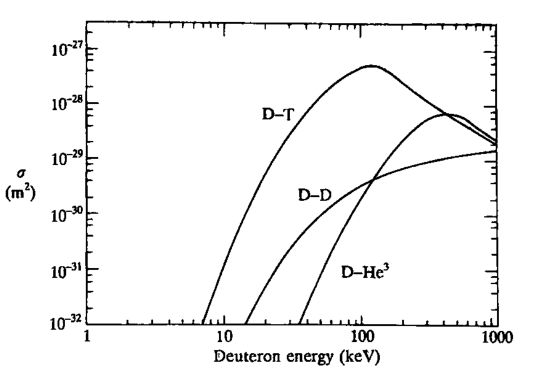
\includegraphics[width=0.7\textwidth]{figures/cross-sections.png}
		\caption{Adapted from \cite{wesson_campbell_tokamaks_2011} Cross-sections for the reactions D-T, D-D and D-$^3$He. The two D-D reactions have similar cross-sections, the graph gives their sum. At 100keV, D-T reaction has the largest cross-section, meaning that more fusion reactions happen in D-T reaction compare to the other two reactions.}
		\label{fig:cross-sections}
	\end{figure}
\end{frame}

\begin{frame}{Thermonuclear Fusion}
	The reaction rate is given by
	\begin{equation}
		R = \left(\frac{8}{\pi}\right)^{1/2}n_1n_2\left(\frac{\mu}{T}\right)^{3/2}\frac{1}{m_1^2}\int \sigma(\epsilon)\epsilon\exp(-\frac{\mu\epsilon}{m_1T})d\epsilon
		\label{eq:reaction-rate}
	\end{equation}
	where the subscript 1 and 2 are D and T, respectively. And $n$ is the number density, $\mu=m_1m_2/(m_1+m_2)$ is the reduced mass, and $\epsilon=\frac{1}{2}m_1(v_1-v-2)^2$ is the kinetic energy of D.
	\begin{itemize}
		\item The rate is maximized when $n_1=n_2$.
		\item The cross-section $\sigma$ is given by Fig.\ref{fig:cross-sections}.
	\end{itemize}
\end{frame}

\begin{frame}{$\expval{\sigma v}$}
	\begin{figure}
		\centering
		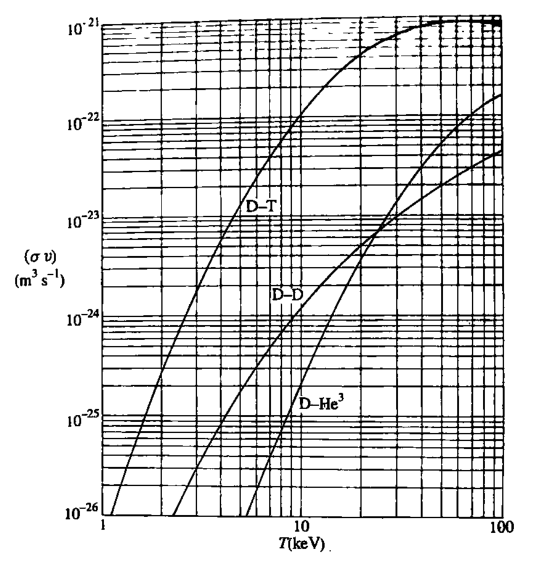
\includegraphics[width=0.4\textwidth]{figures/sigma-v.png}
		\caption{Adapted from \cite{wesson_campbell_tokamaks_2011}, $\expval{\sigma v}$ for D-T, D-D(total) and D-$^3$He reactions as a function of plasma temperature. $\expval{\sigma v}$ for D-D and D-$^3$He are much smaller than that of D-T.}
		\label{fig:sigma-v}
	\end{figure}
\end{frame}
\section{Ignition}
\begin{frame}{Power Balance - Thermonuclear Power}
	For D-T reaction (assuming $n_d=n_t$), the thermonuclear power density is given by
	\begin{equation}
		p_{Tn} = \frac{1}{4}n^2\expval{\sigma v}\varepsilon
		\label{eq:thermonuclear-power-density}
	\end{equation}
	where $n=n_d+n_T$ is the total number of density, and $\expval{\sigma v}$ is drawn in Fig.\ref{fig:sigma-v}, $\varepsilon$ is the energy released per reaction.

	\begin{itemize}
		\item 4/5 of the reaction energy, $\varepsilon$, is carried away by neutrons, the rest is carried by $\alpha$-particles, $\varepsilon_\alpha$.
		\item Neutrons will leave plasma without any interaction.
		\item The $\alpha$-particles will be confined by magnetic field, hence self heating the plasma.
	\end{itemize}
\end{frame}

\begin{frame}{Power Balance - $\alpha$-particle Heating}
	Since the $\alpha$-particles are trapped by the magnetic field, so they will transfer their 3.5MeV energy to the plasma through collisions. Thus, the $\alpha$-particle heating power
	\begin{equation}
		P_\alpha = \int \frac{1}{4}n^2\expval{\sigma v}\varepsilon_\alpha \dd[3]{x} = \frac{1}{4}\overline{n^2\expval{\sigma v}}\varepsilon_\alpha V
		\label{eq:power-alpha}
	\end{equation}
	where the bar means average in the plasma, and $V$ is the volume of the plasma.
\end{frame}

\begin{frame}{Power Balance - Energy Loss}
	Since each plasma particle has energy $3T/2$ ($T/2$ in each degree of freedom), and there are equal number of electrons and ions, so the total energy of the plasma is
	\begin{equation}
		W = \int 3nT\dd[3]{x} = 3\overline{nT}V
	\end{equation}
	where $V$ is the volume of the plasma.

	If the energy confinement time is $\tau_E$, then the energy loss power is
	\begin{equation}
		P_L = W/\tau_E
		\label{eq:power-loss}
	\end{equation}

	\begin{itemize}
		\item To experimentally determine $\tau_E$, we can maintain a steady state plasma by external heating. In this case the power of energy loss can be estimated by the power of heating, $P_L = P_H$, so
		      \[ \tau_E = W/P_H \]
	\end{itemize}
\end{frame}

\begin{frame}{Ignition - Condition}
	The requirement for the plasma burn to be self-sustaining is
	\begin{equation}
		P_\alpha > P_L
	\end{equation}
	Take constant density and temperature for simplicity, we have
	\begin{equation}
		n\tau_E > \frac{12 T}{\expval{\sigma v} \varepsilon_\alpha}
	\end{equation}
	The right-hand-side of the inequality is drawn in Fig.\ref{fig:ignition-condition}.

	Since $\tau_E$ itself is also a function of temperature, so there is a more convenient form,
	\begin{equation}
		nT\tau_E > 3\times10^{21} \text{keV\cdot s}
	\end{equation}
\end{frame}

\begin{frame}{Ignition - Condition}
	\begin{figure}
		\centering
		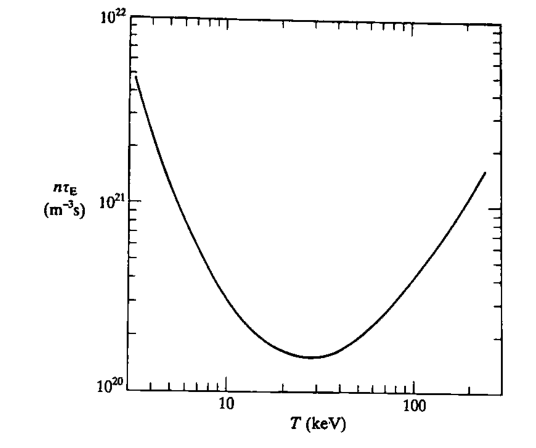
\includegraphics[width=0.6\textwidth]{figures/ignition-condition.png}
		\caption{Adapted from \cite{wesson_campbell_tokamaks_2011}. The value of $n\tau_E$ required to obtain ignition, as a function of temperature.}
		\label{fig:ignition-condition}
	\end{figure}
\end{frame}

\begin{frame}{Ignition - Approach}
	\begin{itemize}
		\item L-mode: Low confinement mode. Poor confinement in this regime.
		\item H-mode: High confinement mode. $\tau_E$ of plasma is long in this regime.
		\item With high enough applied power, plasma transition from L to H-mode.
		\item Once the mode transition happens, the plasma burn is self-sustaining.
	\end{itemize}
	\begin{figure}
		\centering
		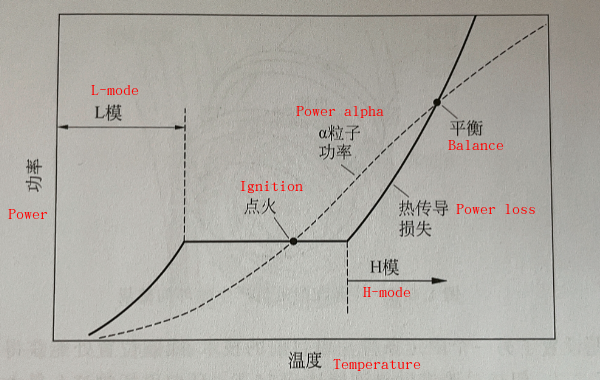
\includegraphics[width=0.6\textwidth]{figures/ignition-approach.png}
		\caption{Adapted from \cite{wesson_campbell_tokamaks_2011}. $P_L$ and $P_\alpha$ as function of temperature.}
	\end{figure}
\end{frame}
\section{Tokamaks}
\begin{frame}{Tokamaks}
    The Tokamak uses coils to control the plasma in the torus-shape chamber.
    \begin{figure}
        \begin{subfigure}{0.5\textwidth}
            \centering
            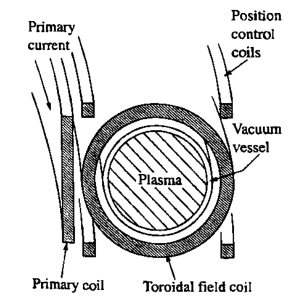
\includegraphics[width=\textwidth]{figures/tokamak-coils.png}
            \caption{Arrangement of coils in a tokamak.}
        \end{subfigure}%
        \begin{subfigure}{0.5\textwidth}
            \centering
            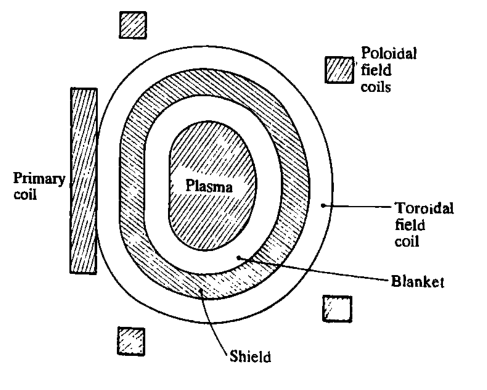
\includegraphics[width=\textwidth]{figures/tokamak-coils-layout.png}
            \caption{Blanket (compound containing Li) is used to absorb the thermonuclear energy and also for tritium breeding.}
        \end{subfigure}
    \end{figure}
\end{frame}

\begin{frame}{Magnetic Field}
    The poloidal and toroidal magnetic field are essential to stabilize the plasma
    \begin{figure}
        \centering
        \begin{subfigure}{0.45\textwidth}
            \centering
            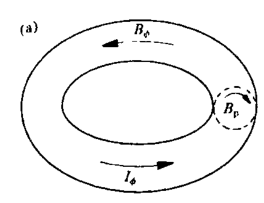
\includegraphics[width=\textwidth]{figures/tokamak-magnetic-field-a.png}
            \caption{Toroidal magnetic field $B_\phi$, and poloidal magnetic field $B_p$ due to toroidal current $I_\phi$.}
        \end{subfigure}%
        \begin{subfigure}{0.45\textwidth}
            \centering
            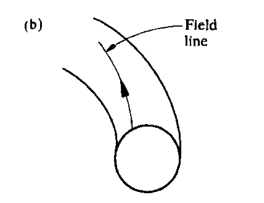
\includegraphics[width=\textwidth]{figures/tokamak-magnetic-field-b.png}
            \caption{Combination of $B_\phi$ and $B_p$ causes field lines to twist around plasma.}
        \end{subfigure}
    \end{figure}
\end{frame}

\begin{frame}{Tokamak Reactor - Structure}
    In the classical design of tokamak reactor, we only replace the energy source by a tokamak, for the rest of the structure we have mature industrial solutions already.
    \begin{figure}
        \centering
        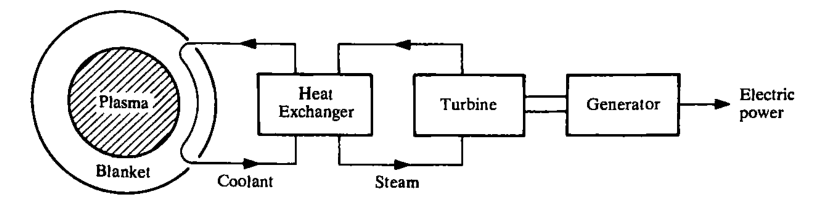
\includegraphics[width=\textwidth]{figures/tokamak-reactor.png}
        \caption{Thermonuclear power absorbed in blanket would be converted into electric power by conventional means.}
    \end{figure}
\end{frame}

\begin{frame}{Tokamak Reactor - Power}
    The power density of the D-T reaction is given by Eq.(\ref{eq:thermonuclear-power-density}), so
    \begin{equation}
        P = \frac{\pi}{2}\varepsilon \int n^2\expval{\sigma v}R dS
    \end{equation}
    where $S$ is an area element of the poloidal cross-section. We can simplify it by taking $R$ as constant and $\bar{a}=(ab)^{1/2}$. Moreover, $\expval{\sigma v}$ can be approximated by $1.1\times 10^{-24} T^2$, and the pressure profile can be taken as $nT = \hat{n}\hat{T}(1-r^2/\bar{a}^2)^\nu$, so the total power
    \begin{equation}
        P = \frac{0.15}{2\nu+1}Rab\left(\frac{\hat{n}}{10^20}\right)^2\hat{T}^2
    \end{equation}
    where the unit of $\hat{T}$ is keV.
\end{frame}

\begin{frame}{Tokamak Reactor - Impurities}
    There are two types of impurities:
    \begin{itemize}
        \item Ions coming from solid surfaces (walls). Need to avoid this since it causes plasma energy loss through radiation.
        \item $\alpha$-particles, $^4$He. The $\alpha$-particles are the byproduct of fusion reaction. It is believed that a magnetic divertor is required to guide the "helium ash" to a "target" surface well separated from the plasma, and to restrict the impurity back-flow.
    \end{itemize}
\end{frame}

\section{Commercial Fusion}
\begin{frame}{Commercial Fusion}
    \begin{itemize}
        \item I will talk about General Fusion's fusion reactor.
        \item I think it is useful to include a list of companies working on fusion energy.
              \url{https://en.wikipedia.org/wiki/Commercial_fusion}
        \item General Fusion uses a structure called Magnetized Target Fusion.
    \end{itemize}
\end{frame}

\begin{frame}{General Fusion - Magnetic Target Fusion}
    \begin{figure}
        \centering
        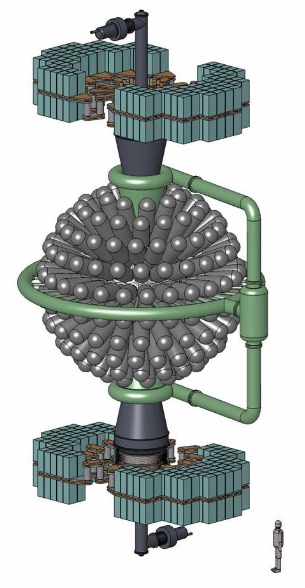
\includegraphics[width=0.3\textwidth]{figures/gf-structure.png}
        \caption{\cite{DelageM.2012PtaM} General Fusion's Acoustic Magnetized Target Fusion Reactor Concept.}
    \end{figure}
\end{frame}

\begin{frame}{General Fusion - Plasma in Field-Reverse Configuration}
    \begin{itemize}
        \item Plasma injectors inject spheromaks with opposite helicity into the center.
        \item Spheromaks meet and form a plasma that is in field reverse configuration (FRC).
        \item Plama in FRC is stable, so no need for the coils. \cite{LabergeMichel2009ERfa}
    \end{itemize}

    \begin{figure}
        \centering
        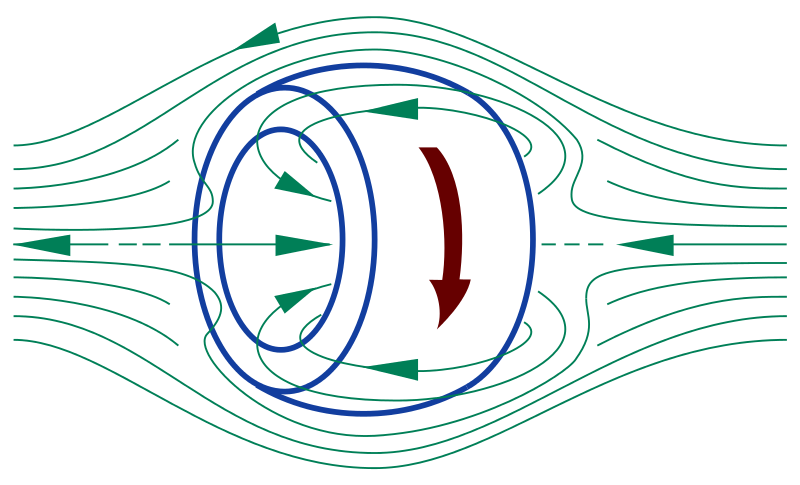
\includegraphics[width=0.3\textwidth]{figures/frc.png}
        \caption{Field-reversed configuration: a toroidal electric current is induced inside a cylindrical plasma, making a poloidal magnetic field, reversed in respect to the direction of an externally applied magnetic field. The resultant high-beta axisymmetric compact toroid is self-confined. Taken from \url{https://commons.wikimedia.org/wiki/File:Field-Reversed_Configuration.svg}}
    \end{figure}
\end{frame}

\begin{frame}{General Fusion - Liquid Pb-Li as Blanket}
    In order to absorb the neutrons emitted from the fusion reaction, a liquid metal, Pb-Li, is used as the blanket. Moreover, the Li element can help to breed the tritium through the reaction, $^7Li+n \to ^4He + ^3H + n$, for further fusion reaction. \cite{LabergeMichel2009ERfa}
    \begin{itemize}
        \item Pb-Li liner is spun up in the device to wrap the plasma.
        \item Steam piston compresses all the things to create fusion.
        \item Liquid metal liner is extracted for heat exchange purpose.
    \end{itemize}

    \begin{figure}
        \centering
        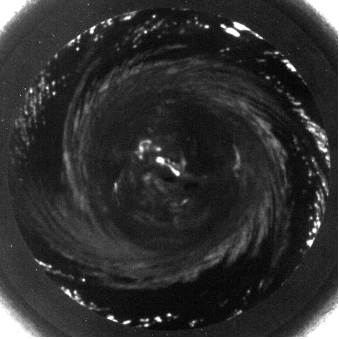
\includegraphics[width=0.3\textwidth]{figures/liquid-pb.png}
        \caption{Image of Liquid Pb.}
    \end{figure}
\end{frame}

%%%%%%%%%%%%%%%%%%%%
% references
%%%%%%%%%%%%%%%%%%%%
\newpage
\begin{frame}[allowframebreaks]
	\bibliographystyle{abbrv}
	\bibliography{../references}
	\nocite{*}
\end{frame}

\end{document}
